\section{Background and Motivation}
\label{sec:bg}
%The hypervisor cache can be used in many different ways in a virtualized
%system~\cite{kvmzcache}.
%
With the Linux+KVM virtualization solution page cache of the
host operating system acts as an inclusive cache.
%For example, page cache of the Linux host in a KVM virtualization platform 
%can act as an inclusive cache in the disk IO access path.
%
Previous studies~\cite{kvmzcache,singleton} have shown that
inclusive caching can be wasteful due to duplication of disk blocks 
across the VMs and the host. 
%
In this paper, we focus on exclusive cache designs~\cite{memtrans} 
like transcendent memory~\cite{memtrans} 
where a symbiosis is proposed between 
the page caches of virtual machines and the hypervisor managed
second chance cache.
%implemented in the hypervisor. 

%\begin{figure}[t]
%\centering
%\begin{subfigure}[b]{0.35\textwidth}
%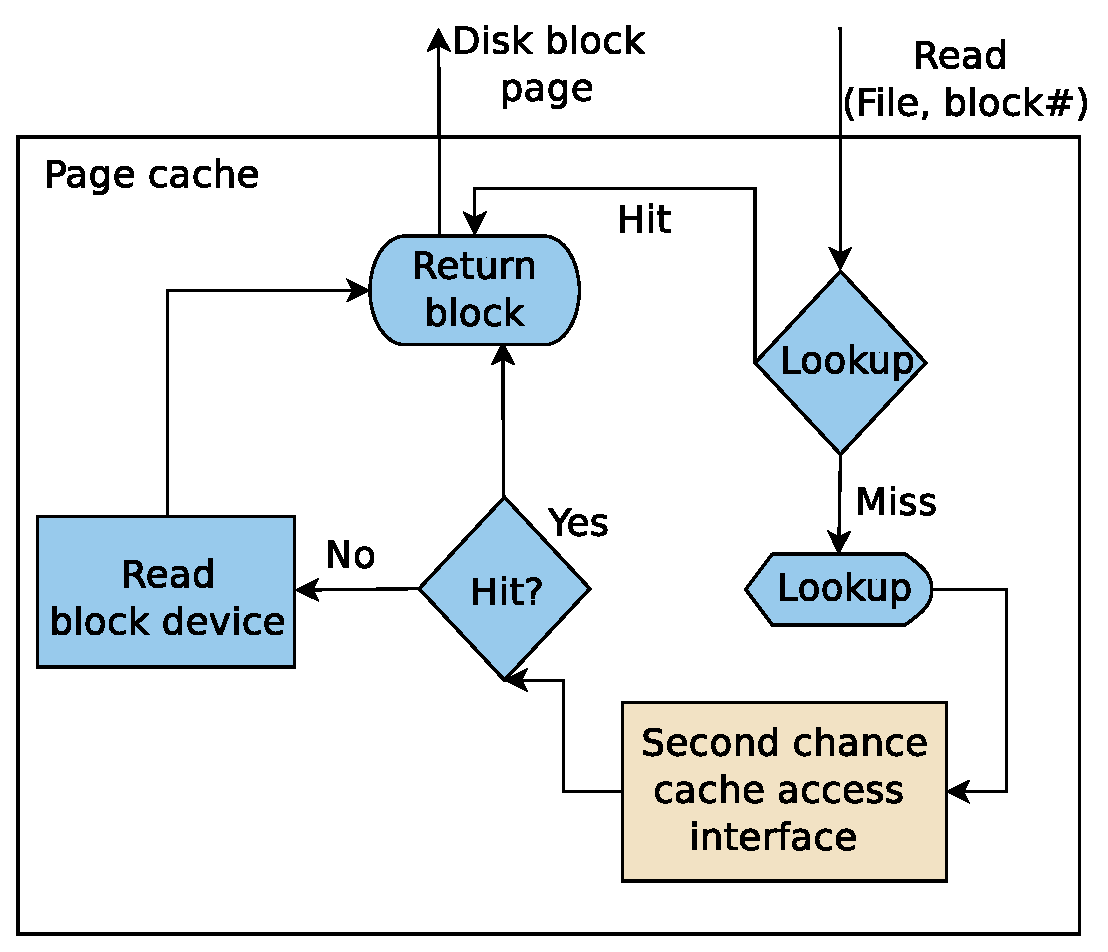
\includegraphics[width=\textwidth]{images/cc_get}
% \caption{Cache lookup of file block}
%\vspace{0.25cm}
% \label{fig:cc_get}
%\end{subfigure}

%\begin{subfigure}[b]{0.35\textwidth}
%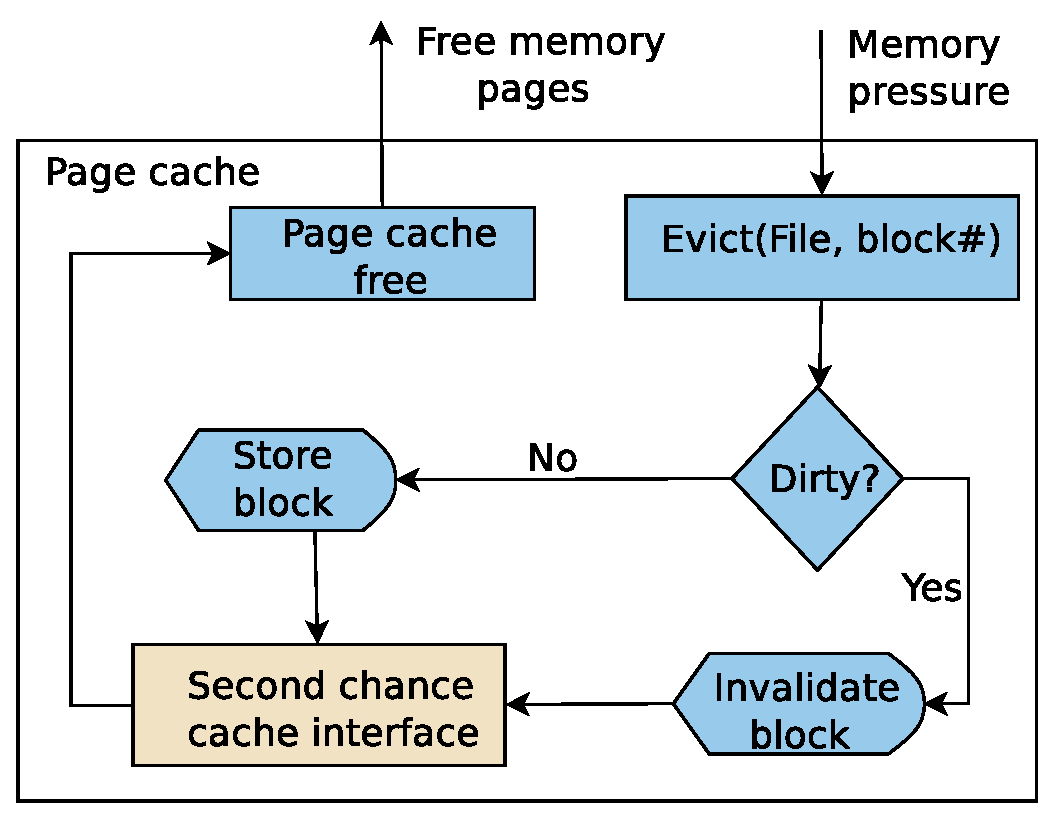
\includegraphics[width=\textwidth]{images/evict}
% \caption{Cache eviction of a file block}
% \label{fig:cc_evict}
%\end{subfigure}

%\caption{Operational view of second chance cache integration
%         with page cache.}
% \label{fig:cleanache_ops}
%\end{figure}

\subsection{Exclusive second chance caching}
\label{subsec:hcache}

\begin{figure}[t]
\centering
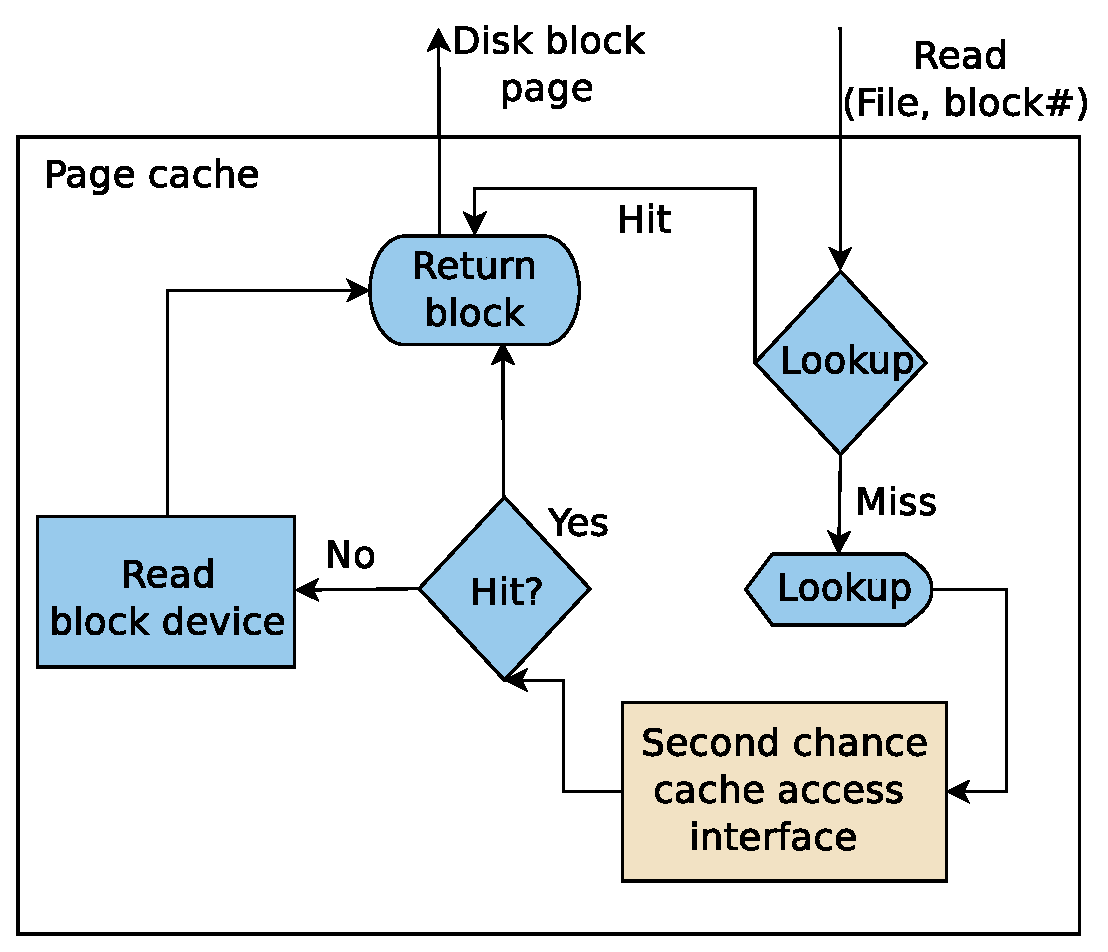
\includegraphics[width=0.35\textwidth]{images/cc_get}
 \caption{Cache lookup of file blocks in the page cache-second chance
cache integrated caching systems.}
 \label{fig:cc_get}
\vspace{-0.4cm}
\end{figure}


%
%\puru{Three figures is a too much for a subsection of the background.
%2a is the one to keep. Also 2a needs updates.}

%In Figure~\ref{fig:scache}, architecture of exclusive second chance cache
%is shown.
%%
%User space application initiated file IO requests are first looked up in the 
%operating system page cache to serve the requests without performing disk IO.
%%
With an exclusive second chance cache, application initiated file IO
requests are looked up in the OS managed disk page cache.
%
On a page cache miss, requests
are queried (lookup operation) in the second-chance cache (Figure~\ref{fig:cc_get}).
%
The second chance cache interface is tightly integrated with the page cache layer
and extends the IO path.
%to perform disk block lookup in the second chance cache in case of a page cache
%lookup failure.
%
When a clean disk block is evicted from page cache, a store operation is
initiated through the second chance cache interface.
%
To maintain exclusivity between the two caches, a block evicted from the
page cache is stored into the second chance cache and a block read from 
the second chance cache is removed from the second chance cache
and transferred to the page cache.

%
A generic second chance cache interface is implemented through 
%an actual 
%cache store implementation (Figure~\ref{fig:scache}) with choice of storage 
a cache store implementation using a storage option
(e.g., memory or SSD), storage optimizations (e.g., compression, deduplication) 
and, cache management policies for eviction and cache partitioning.
%
Linux \cleancache~\cite{cleancache}, an abstract second chance cache 
access interface, provides a generic second chance cache integration 
framework with the page cache.
%
The key operations of the interface are:---lookup (\get)
a disk block, store (\put)  a block in the cache and \flush{}
to invalidate objects from the cache (refer to Figure~\ref{fig:scache}).
%
In a virtualized setup, where second chance cache is implemented in the hypervisor, 
above operations ensure exclusive caching between the guest disk cache and
the hypervisor cache.
%
Hypervisor managed caches interface with the guest OS second chance
cache interface using
%hypervisor interfaces like hypercall (VMCALL)
the hypercall (VMCALL) API (Figure~\ref{fig:scache}).
%
The second chance stores only clean pages evicted from the page cache
and is indexed based on file system mount points or virtual machine
identifiers, the file information and the block number.
%
Several second chance cache implementations for native Linux and for
different virtualization solutions 
exist~\cite{zcache, oracletmem,kvmzcache, mortar}.
%
However, no state-of-the-art solution
supports application cognizant second chance cache management,
especially for nested hosting setups.
\begin{figure}[t]
  \centering
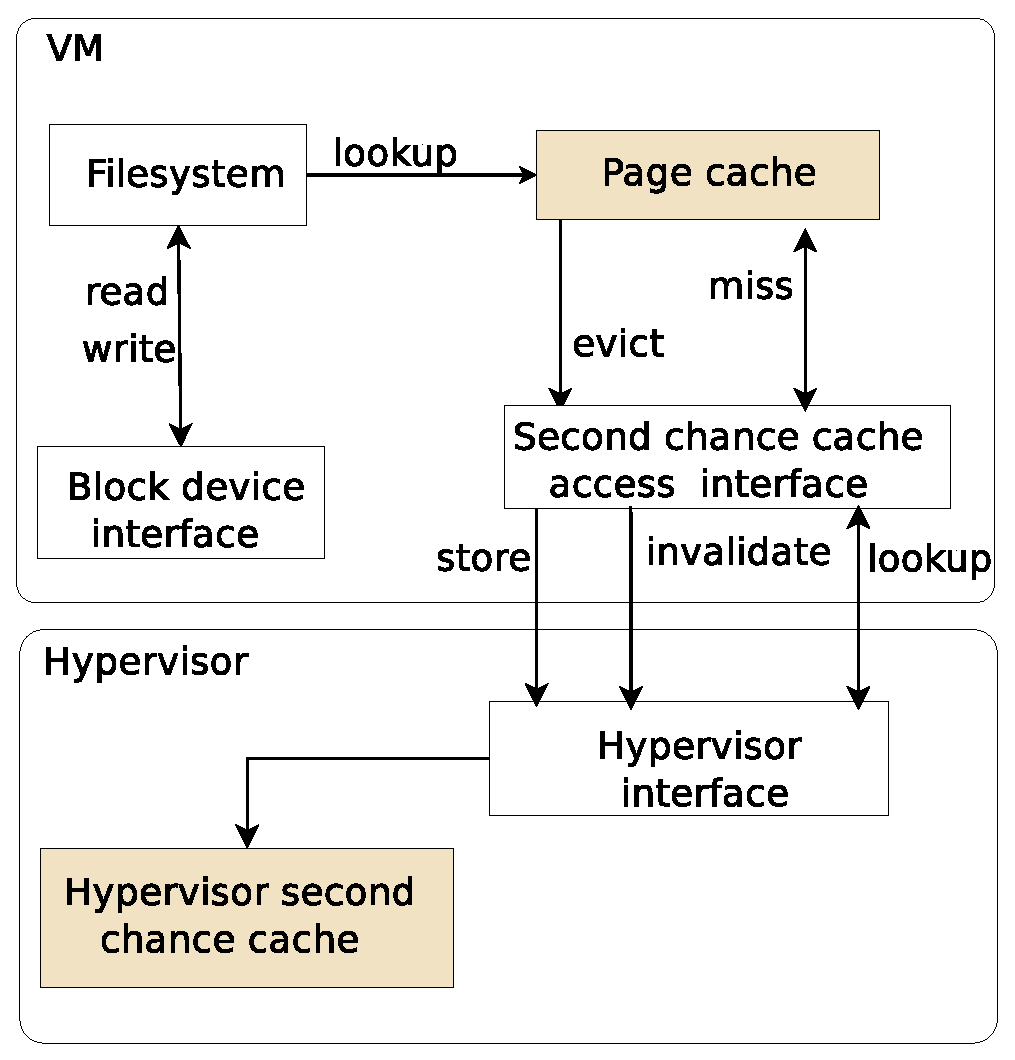
\includegraphics[width=0.35\textwidth]{images/tmem}
 \caption{Overview of second chance cache integration with OS page cache 
with exclusive mode of operation.}
 \label{fig:scache}
\vspace{-0.2cm}
\end{figure}
%can be part of the operating system (e.g., \zcache{} in
%the Linux OS~\cite{zcache}) or part of the hypervisor in a virtualized 
%system~\cite{oracletmem,kvmzcache,mortar}. 
%
%
%The block device interface is used as the last resort to access blocks from the disk
%on cache lookup failure at both the page cache and the second chance cache.
%
%\subsubsection{Exclusive second chance cache operations}
%\label{subsec:hcache}

%Transcendent memory (or \tmem{})~\cite{oracletmem} is a state-of-the-art
%hypervisor-managed cache which implements exclusive caching by
%design~\cite{memtrans}.
%
%The \tmem{} cache stores \emph{clean} disk pages
%does not contain dirty data at any
%point in time 
%and thus is transparent to storage durability mechanisms.
%
%An example hypervisor caching framework (illustrated in Figure~\ref{fig:tmem}) 
%has three major components---(i) a guest OS \cleancache{} interface, (ii) a hypervisor 
%managed back-end cache, and (iii) a hypervisor interface to access the cache.
%
%On a disk page lookup failure in the first chance cache (page cache),
%second chance cache  lookup (a \get{} operation) is performed 
%to {\em find-and-fetch} the requested block from the second chance cache 
%onto the page cache as shown in Figure~\ref{fig:cc_get}.
%%
%If the block is not found in the second chance cache, a block IO request is
%initiated to fetch the block from the block device.
%
%Similarly, when the page cache layer is requested to evict clean/unmodified cached 
%disk blocks, the block is stored in the second chance cache (a.k.a \put{} operation)
%(Figure~\ref{fig:cc_evict}). 
%%
%%For a dirty block eviction, second chance cache invalidate (\flush) operation
%purges the page from the second chance cache, if present, since the second chance
%cache version of the page is now outdated.
%
%

%The unique key provided by the \cleancache{} abstract interface is a three 
%tuple i.e., file system mount point ID (\texttt{pool-id}), 
%file identifier (\texttt{inode number}) and the block offset of the requested 
%file block.
%%cache provides a key-value interface for storing page
%%objects.
%%
%The second chance cache store is responsible for mapping these keys to actual
%storage objects to implement \get, \put{} and \flush{} operations.
%%
%%The \texttt{pool-id} is negotiated during the file system initialization. 
%
%In a hypervisor cache implementation, the hypervisor cache is additionally responsible
%to uniquely identify requests from different VMs which is typically ensured by extending the 
%key with an additional \texttt{vm-id} element.

\subsection{Application container isolation framework}
%
Light-weight resource isolation frameworks like Linux control 
groups (\cgroup)~\cite{cgroup} provide performance isolation 
across multiple execution domains with low virtualization 
and multiplexing overheads compared to hypervisor enabled 
system virtualization solutions.
%machine level isolation solutions.
%
Linux \cgroup~\cite{cgroup} and FreeBSD Jails~\cite{jail} are examples
of performance isolation frameworks facilitating resource management 
for a group of processes by specifying group-level resource limits.
%for different
%resources e.g., CPU time, memory size, network and disk bandwidth etc..
%
%For example, to manage memory across \cgroups, two control knobs 
%i.e., \texttt{hard limit} and \texttt{soft limit} are provided in Linux \cgroup{}
%resource control model.
%
Using the process grouping based isolation model, container management
solutions like LXC~\cite{lxc} and Docker~\cite{docker} enable hosting
multiple applications in different application groups (containers).
%

%In a nested hosting system like derivative clouds, the two resource control 
With containers in virtual machines derivative clouds, 
the two resource controllers---the hypervisor and the \cgroup{} subsystem---operate 
in an agnostic manner w.r.t. each other.
%
As a result, centralized/global hypervisor cache 
distribution from the containers perspective is not 
deterministic (\S\ref{subsec:motivation}).
%is uncontrolled and arbitrary (\S\ref{subsec:motivation}).
%
To enable differentiated partitioning of the hypervisor cache and 
to facilitate intelligent use of multiple storage backends across 
containers, it is necessary to design a
solution that can provide synergy across the two control points.
%

\subsection{Motivation}
\label{subsec:motivation}
%\begin{figure*}
%\centering
%\begin{subfigure}{0.5\columnwidth} 
%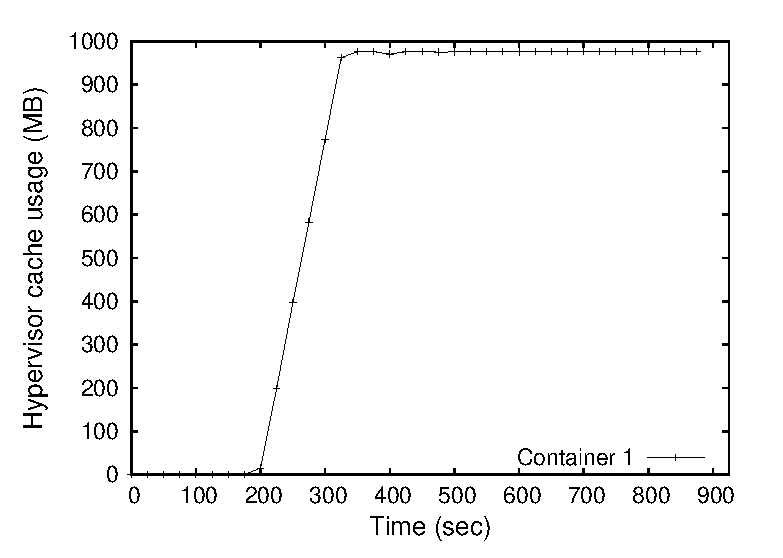
\includegraphics[width=\columnwidth]{data/motivation/disparity_c1} 
% \caption{Application container 1}
% \label{fig:cachedistrib1} 
%\end{subfigure} \hfill
%
%\begin{subfigure}{0.5\columnwidth}
%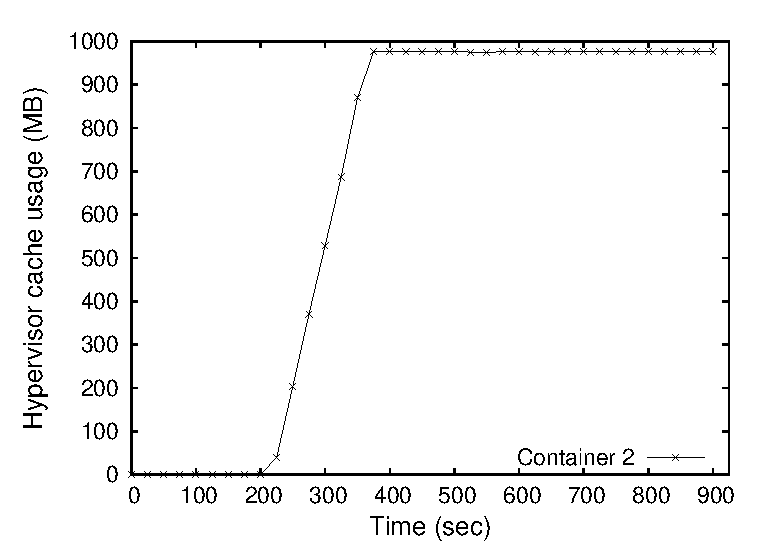
\includegraphics[width=\columnwidth]{data/motivation/disparity_c2} 
% \caption{Application container 2}
% \label{fig:cachedistrib2} 
%\end{subfigure} \hfill
%
%\begin{subfigure}{0.5\columnwidth}
%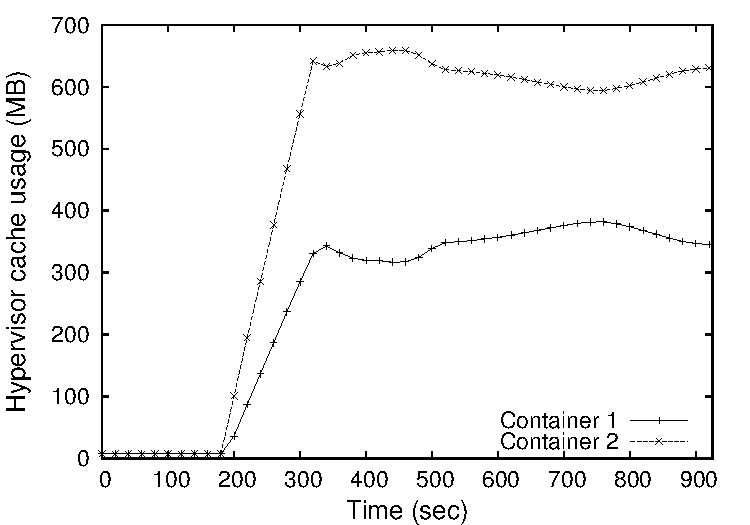
\includegraphics[width=\columnwidth]{data/motivation/disparity1}
% \caption{Application containers 1 and 2}
% \label{fig:cachedistrib12} 
%\end{subfigure} \hfill
%
%\begin{subfigure}{0.5\columnwidth}
%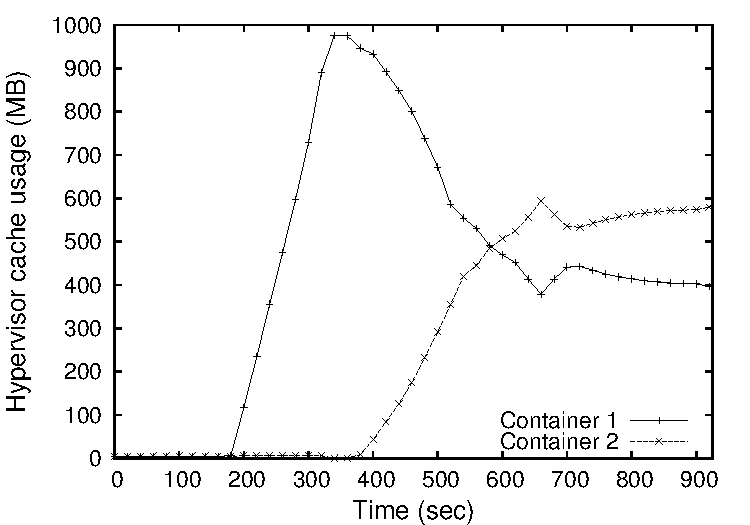
\includegraphics[width=\columnwidth]{data/motivation/disparity2}
% \caption{Application containers 1 and 2}
% \label{fig:cachedistrib12_offset} 
%\end{subfigure} \hfill
%
%\caption{Hypervisor cache distribution across two containers hosted inside a VM.}
%\label{fig:cachedistrib}
%\end{figure*}
\begin{figure}
\centering
\begin{subfigure}{0.49\columnwidth} 
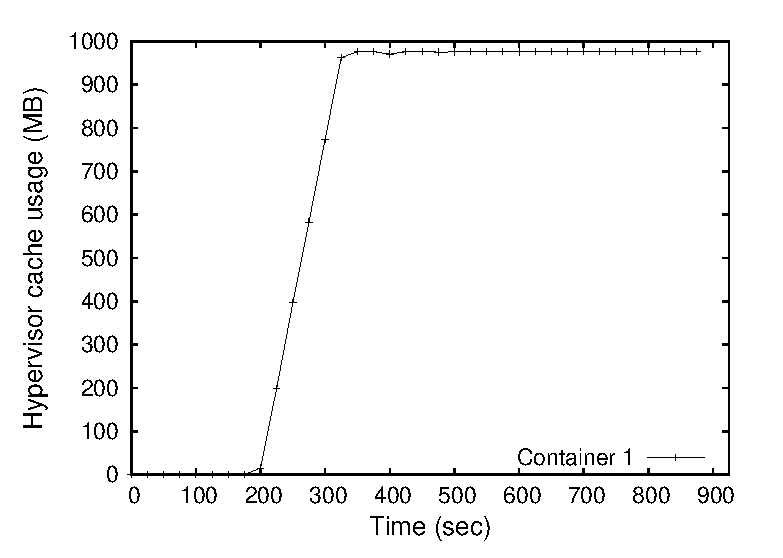
\includegraphics[width=\columnwidth]{data/motivation/disparity_c1} 
 \caption{Application container 1}
 \label{fig:cachedistrib1} 
\end{subfigure} \hfill
%
\begin{subfigure}{0.49\columnwidth}
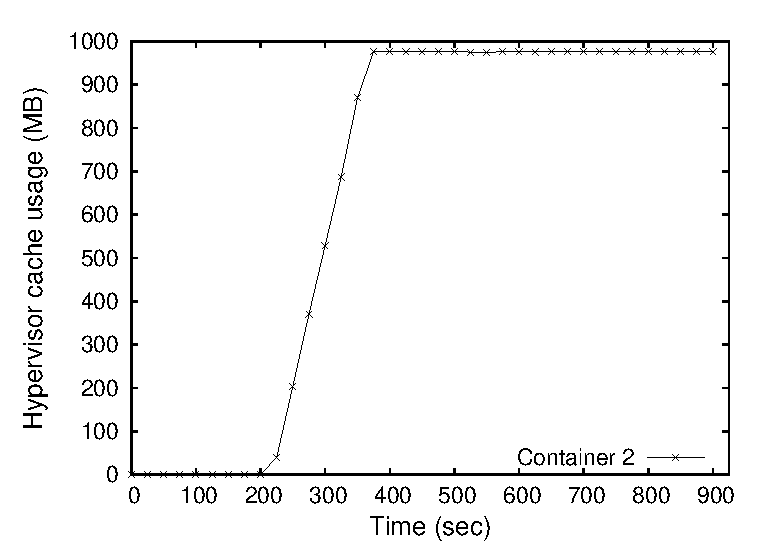
\includegraphics[width=\columnwidth]{data/motivation/disparity_c2} 
 \caption{Application container 2}
 \label{fig:cachedistrib2} 
\end{subfigure} \hfill
%
\caption{Hypervisor cache distribution when application containers
         executed separately.}
\vspace{-0.3cm}
\label{fig:separate}
\end{figure}


\begin{figure}
\centering
\begin{subfigure}{0.49\columnwidth}
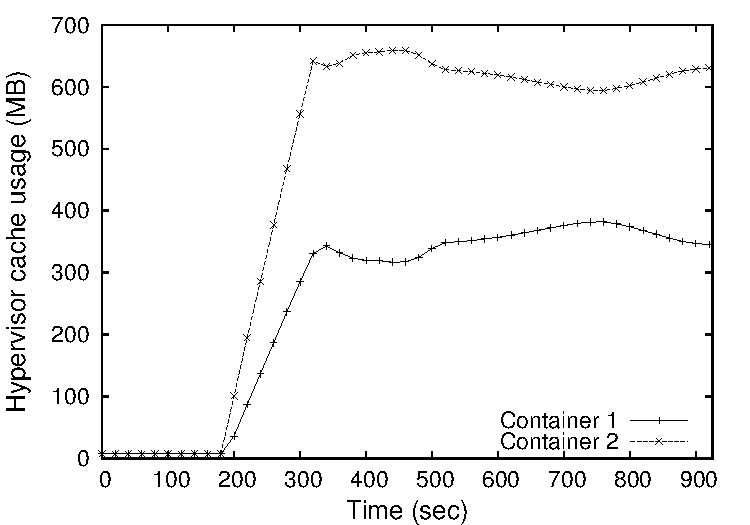
\includegraphics[width=\columnwidth]{data/motivation/disparity1}
 \caption{Same start time}
 \label{fig:cachedistrib12} 
\end{subfigure} \hfill
%
\begin{subfigure}{0.49\columnwidth}
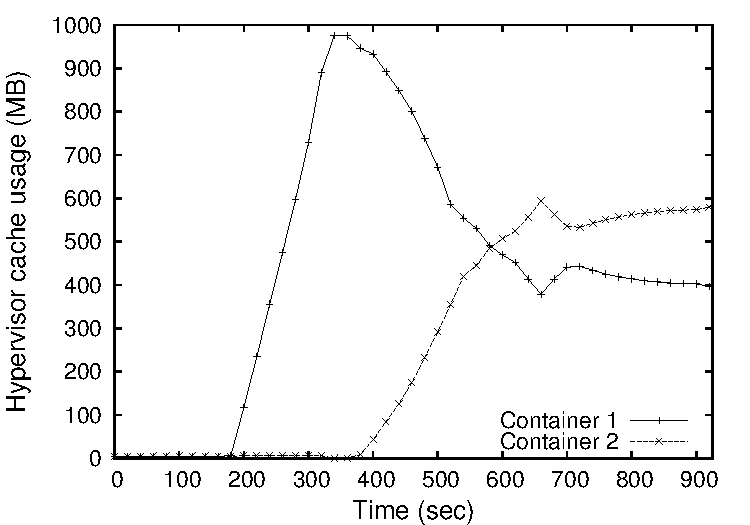
\includegraphics[width=\columnwidth]{data/motivation/disparity2}
 \caption{Container 2 offset by 200 sec}
 \label{fig:cachedistrib12_offset} 
\end{subfigure} \hfill
%
%\caption{Hypervisor cache distribution when application containers
%         executed simultaneous with different application start times.}
\caption{Hypervisor cache distribution with different start times of
application containers.}
\vspace{-0.4cm}
\label{fig:together}
\end{figure}


To demonstrate the non-deterministic cache distribution in a nested 
container setup, we performed an experiment with a VM configured 
with 2GB memory and 4 VCPUs on a host with 32GB memory and 16 CPUs.
%
The hypervisor cache 
was not cognizant of the containers and its size was limited to 1GB.
%was similar to Xen tmem~\cite{oracletmem} which
% i.e., cache limit enforcement was on a per-VM basis.
%
%The maximum hypervisor cache limit was set to 1GB for this experiment.
%
Two application containers (Container 1 and Container 2) configured with 
the same memory limits (through \cgroup) executed the \web-workload of the 
\file~workload suite~\cite{filebench}.
%
The only difference between the two containers was their IO load; 
Container 1 executed two
\web~threads while Container 2 executed three \web-threads.
%

With this setup, when Container 1 and Container 2 executed separately one-at-a-time, 
each of them used up the entire hypervisor cache (Figure~\ref{fig:separate}).
%as shown in 
%Figure~\ref{fig:cachedistrib1} and Figure~\ref{fig:cachedistrib2}, respectively.
%
The implication being that each application is capable of taking advantage 
of the configured hypervisor cache to its capacity when executed separately.
%
%To show the non-deterministic cache distribution behavior, we performed an 
%experiment with the same setup where both application containers shared the 
%hypervisor cache during
%the workload execution.
%

When both applications were started simultaneously,
the hypervisor
cache was distributed across containers in a disproportionate manner.
%
Share of Container 2 was approximately two times that of
Container 1 as shown in Figure~\ref{fig:cachedistrib12}.
%
The non-determinism is a side-effect of the IO load and
the FIFO-based global eviction policy (not ensuring container level fairness) 
of the hypervisor cache.
%
%In another hypervisor cache sharing experiment (Figure~\ref{fig:cachedistrib12_offset}),
When Container 2 started executing its  workload after a delay of 200 seconds 
form start of workload in Container 1,
%that of container 1 application start time.  
%
%In this case, container 1 dominated the cache usage in initial part, after which
Container 1 dominated the cache usage till about 500 seconds, after which
cache share of Container 2 increased before surpassing that of 
Container 1 at around 600 seconds(Figure~\ref{fig:cachedistrib12_offset}).
%
%\puru{maybe we should add a table to compare performance with
%deterministic cache sizing.}
%These results demonstrate the non-determinism in cache distribution across 
%application containers executing inside the VMs
%, specifically in case of derivative 
%cloud setups.
%
%Therefore, 
These results demonstrate that state-of-the-art hypervisor caches are unable to
implement policies (e.g., fair allocation to application containers) in a 
deterministic manner at a sub-VM granularity.
%

\subsubsection{VM level memory management flexibility}
\label{subsec:sdc}
%
%
\begin{figure}[t]
  \centering
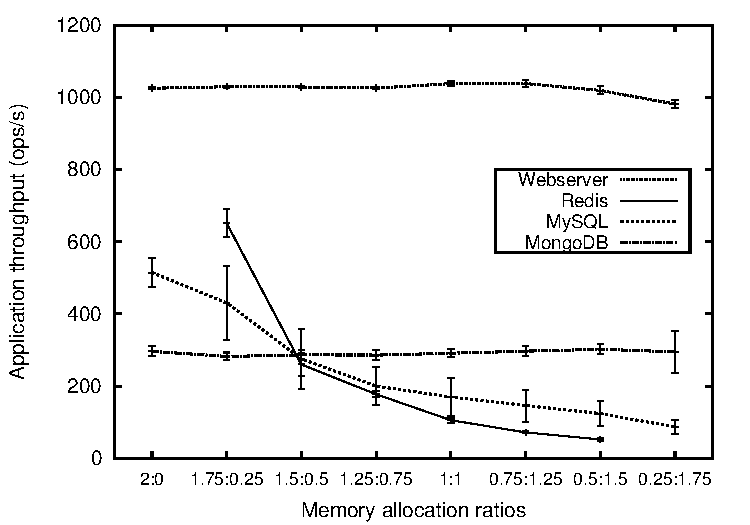
\includegraphics[width=0.45\textwidth]{images/appl_behavior} 
 \caption{Application performance with different provisioning configurations 
  at the two levels of a derivative cloud.}
 \label{fig:app_behavior} 
\end{figure}
%
To analyze the impact of memory provisioning at the two 
levels (guest OS and hypervisor cache) in a nested setup and motivate the need for 
guest OS control on the hypervisor cache sizing, we performed the 
following experiment.
%
2GB memory was split in different ratios to allocate memory for the container 
inside the VM (through Cgroups) and the hypervisor cache.
%
For example, an allocation ratio of 1.5:0.5 (Figure~\ref{fig:app_behavior}) refers to
a 1.5 GB in-VM memory limit and 0.5 GB hypervisor cache limit for
the container. 
%
Application performance for four different workloads,
the Filebench \web{} workload and YCSB~\cite{ycsb} using 
Redis, MongoDB and MySQL data stores,
with different allocation ratios is shown in 
Figure~\ref{fig:app_behavior}. 
%
Application throughput for Webserver and MongoDB remain almost unchanged 
(1000 ops/sec and ~300 ops/sec, respectively) while Redis and MySQL performance 
degraded when more memory was split with the hypervisor cache.
%
Redis was exceptional in extreme split scenarios---very high throughput (10406 ops/sec) was
observed with 2GB VM memory allocated to the container and, application stall observed when 256 MB 
memory was allocated through the Cgroup and rest allocated in the hypervisor cache.
%
\begin{table}[t]
%\scriptsize
\begin{center}
\begin{tabular}{|c|c|c|c|}
\hline
{\bf Application} & {\bf Total} & {\bf Anonymous} & {\bf Hypervisor} \\
{\bf usage } & {\bf swap} & {\bf memory} & {\bf cache} \\
 & {\bf (MB)} & {\bf usage (MB)} & {\bf usage (MB)} \\
\hline 
\hline 
Websever & 0 & 88.9 & 1023 \\
Redis & 996 &  1021 & 18.5 \\
MySQL & 879 & 1013 & 34 \\
MongoDB & 0 & 251 & 1023 \\
\hline 
\end{tabular}
\caption{Guest OS metrics for different applications with equal split (1GB in-VM and 1GB 
         hypervisor cache) scenario.}
\label{table:app_diagnosis}
\vspace{-1cm}
\end{center}
\end{table}

Explanation for the application behavior is presented in 
Table~\ref{table:app_diagnosis}.
%
Applications requiring anonymous memory can not be helped by the 
hypervisor cache and resort back to swapping as the last alternate.
%
For applications depending on file I/O, hypervisor cache 
can offload the caching responsibility without causing any
application degradation.
%
These results show that providing the VM level memory manager with the option
to choose different cache and in-VM memory configurations provides flexibility
to meet various application SLA objectives.

 
%
%Hypervisor caching solutions with application level differentiated 
%management fall short to facilitate decentralized policy enforcement.
Existing centralized hypervisor cache management 
techniques (e.g., Morai~\cite{sdc}, Centaur~\cite{centaur}) have
limitations w.r.t. their applicability in such scenarios.
%
The required flexibility to empower VM-level memory management across
applications (as deduced from the previous experiment) is not supported.
%
For example, existing techniques can neither improve performance of the 
applications that depend on anonymous memory allocations (e.g., Redis) 
nor provide flexibility to free in-VM memory by selectively offloading 
applications (e.g., Webserver) to the hypervisor cache.
%
%Some additional drawbacks in the existing hypervisor caching 
%solutions are mentioned below. 
Additionally, existing hypervisor caching solutions~\cite{sdc,centaur}
%
%First, they operate in an inclusive cache operation mode
operate in an inclusive cache operation mode
w.r.t. the guest OS page cache which is wasteful due to duplicate 
storage of disk blocks in memory.
%
%Second, 
Further, application differentiation at the hypervisor cache is not
generic. For example, Morai~\cite{sdc} requires applications to be 
hosted on different virtual disks so that they can be distinguished at the
hypervisor level.
%


%
To support differentiated policy enforcement in derivative cloud setups
at the nested levels, a rethink of the hypervisor cache design is required.    
%
The proposed design should allow independent memory management at the two 
nested levels with the hypervisor still being the enforcing entity. 
%
